This subsection is used when we have to save or retrive data from the database. When user tries to login, register, add self, add item or search we have to use database. When somebody wants to register for the app, he provides all the infomration then these information is taken by the DB controller and saved in organized manner. same process occurs for all the other activities like adding self, adding item or login.
\subsection{DB Controller}
This is a type of main controller of the Database system. All the data that needs to be stored in database is first handled by this layer and later stored in the database. When any of the other layer send data to the database layer, first database layer takes the information and figures out what type of data is provided and what to do with the given data.

\begin{figure}[h!]
	\centering
 	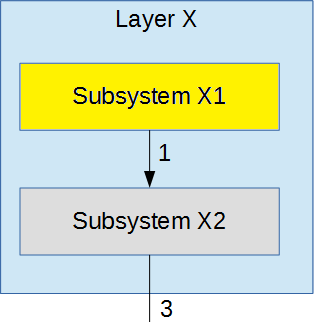
\includegraphics[width=0.60\textwidth]{images/subsystem}
 \caption{Example subsystem description diagram}
\end{figure}

\subsubsection{Assumptions}
These are the following assumptions made about this subsection:
\begin{itemize}
    \item All the input provided to be saved in the database is a valid input.
    \item Device is connected to the internet when saving or retrieving the data.
\end{itemize}

\subsubsection{Responsibilities}
These are the following responsibilities of the Database Controller.
\begin{itemize}
    \item It must be able to take input sent from all the other layers.  
    \item When input is captured it must be able to classify if the data is login data or sign up data. Must be able to classify if the incoming data is trying to search the item or save the item in the database.
\end{itemize}

\subsubsection{Subsystem Interfaces}
Each of the inputs and outputs for the subsystem are defined here. Create a table with an entry for each labelled interface that connects to this subsystem. For each entry, describe any incoming and outgoing data elements will pass through this interface.

\begin {table}[H]
\caption {Subsystem interfaces} 
\begin{center}
    \begin{tabular}{ | p{1cm} | p{6cm} | p{3cm} | p{3cm} |}
    \hline
    ID & Description & Inputs & Outputs \\ \hline
    \#xx & Description of the interface/bus & \pbox{3cm}{input 1 \\ input 2} & \pbox{3cm}{output 1}  \\ \hline
    \#xx & Description of the interface/bus & \pbox{3cm}{N/A} & \pbox{3cm}{output 1}  \\ \hline
    \end{tabular}
\end{center}
\end{table}

\subsection{Login Mgmt}


\begin{figure}[h!]
	\centering
 	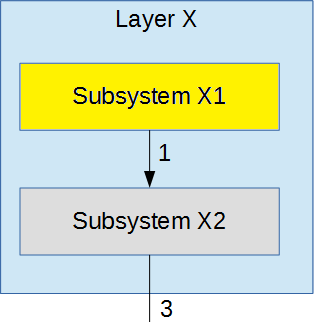
\includegraphics[width=0.60\textwidth]{images/subsystem}
 \caption{Example subsystem description diagram}
\end{figure}

\subsubsection{Assumptions}
These are the following assumptions made about this subsection:
\begin{itemize}
    \item 
\end{itemize}

\subsubsection{Responsibilities}
Each of the responsibilities/features/functions/services of the subsystem as identified in the architectural summary must be expanded to more detailed responsibilities. These responsibilities form the basis for the identification of the finer-grained responsibilities of the layer's internal subsystems. Clearly describe what each subsystem does.

\subsubsection{Subsystem Interfaces}
Each of the inputs and outputs for the subsystem are defined here. Create a table with an entry for each labelled interface that connects to this subsystem. For each entry, describe any incoming and outgoing data elements will pass through this interface.

\begin {table}[H]
\caption {Subsystem interfaces} 
\begin{center}
    \begin{tabular}{ | p{1cm} | p{6cm} | p{3cm} | p{3cm} |}
    \hline
    ID & Description & Inputs & Outputs \\ \hline
    \#xx & Description of the interface/bus & \pbox{3cm}{input 1 \\ input 2} & \pbox{3cm}{output 1}  \\ \hline
    \#xx & Description of the interface/bus & \pbox{3cm}{N/A} & \pbox{3cm}{output 1}  \\ \hline
    \end{tabular}
\end{center}
\end{table}

\subsection{Register Mgmt}
This SubSystem deals with taking the item description from user. Variety of options are provided for inputting the item. User can use the camera in the cellphone to 

\begin{figure}[h!]
	\centering
 	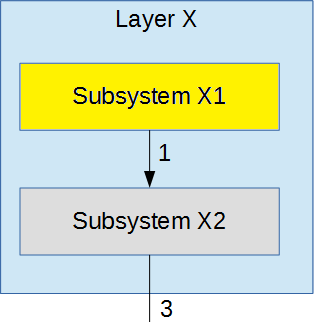
\includegraphics[width=0.60\textwidth]{images/subsystem}
 \caption{Example subsystem description diagram}
\end{figure}

\subsubsection{Assumptions}
These are the following assumptions made about this subsection:
\begin{itemize}
    \item 
\end{itemize}

\subsubsection{Responsibilities}
Each of the responsibilities/features/functions/services of the subsystem as identified in the architectural summary must be expanded to more detailed responsibilities. These responsibilities form the basis for the identification of the finer-grained responsibilities of the layer's internal subsystems. Clearly describe what each subsystem does.

\subsubsection{Subsystem Interfaces}
Each of the inputs and outputs for the subsystem are defined here. Create a table with an entry for each labelled interface that connects to this subsystem. For each entry, describe any incoming and outgoing data elements will pass through this interface.

\begin {table}[H]
\caption {Subsystem interfaces} 
\begin{center}
    \begin{tabular}{ | p{1cm} | p{6cm} | p{3cm} | p{3cm} |}
    \hline
    ID & Description & Inputs & Outputs \\ \hline
    \#xx & Description of the interface/bus & \pbox{3cm}{input 1 \\ input 2} & \pbox{3cm}{output 1}  \\ \hline
    \#xx & Description of the interface/bus & \pbox{3cm}{N/A} & \pbox{3cm}{output 1}  \\ \hline
    \end{tabular}
\end{center}
\end{table}

\subsection{Self Management}
This SubSystem deals with taking the item description from user. Variety of options are provided for inputting the item. User can use the camera in the cellphone to 

\begin{figure}[h!]
	\centering
 	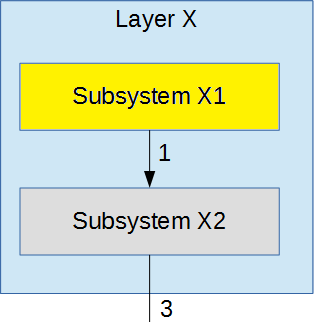
\includegraphics[width=0.60\textwidth]{images/subsystem}
 \caption{Example subsystem description diagram}
\end{figure}

\subsubsection{Assumptions}
These are the following assumptions made about this subsection:
\begin{itemize}
    \item 
\end{itemize}

\subsubsection{Responsibilities}
Each of the responsibilities/features/functions/services of the subsystem as identified in the architectural summary must be expanded to more detailed responsibilities. These responsibilities form the basis for the identification of the finer-grained responsibilities of the layer's internal subsystems. Clearly describe what each subsystem does.

\subsubsection{Subsystem Interfaces}
Each of the inputs and outputs for the subsystem are defined here. Create a table with an entry for each labelled interface that connects to this subsystem. For each entry, describe any incoming and outgoing data elements will pass through this interface.

\begin {table}[H]
\caption {Subsystem interfaces} 
\begin{center}
    \begin{tabular}{ | p{1cm} | p{6cm} | p{3cm} | p{3cm} |}
    \hline
    ID & Description & Inputs & Outputs \\ \hline
    \#xx & Description of the interface/bus & \pbox{3cm}{input 1 \\ input 2} & \pbox{3cm}{output 1}  \\ \hline
    \#xx & Description of the interface/bus & \pbox{3cm}{N/A} & \pbox{3cm}{output 1}  \\ \hline
    \end{tabular}
\end{center}
\end{table}

\subsection{Item Mgmt}
This SubSystem deals with taking the item description from user. Variety of options are provided for inputting the item. User can use the camera in the cellphone to 

\begin{figure}[h!]
	\centering
 	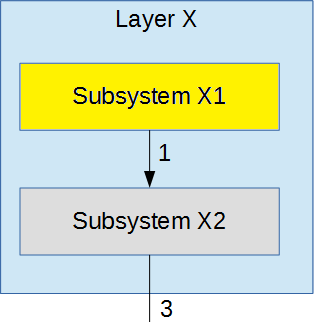
\includegraphics[width=0.60\textwidth]{images/subsystem}
 \caption{Example subsystem description diagram}
\end{figure}

\subsubsection{Assumptions}
These are the following assumptions made about this subsection:
\begin{itemize}
    \item 
\end{itemize}

\subsubsection{Responsibilities}
Each of the responsibilities/features/functions/services of the subsystem as identified in the architectural summary must be expanded to more detailed responsibilities. These responsibilities form the basis for the identification of the finer-grained responsibilities of the layer's internal subsystems. Clearly describe what each subsystem does.

\subsubsection{Subsystem Interfaces}
Each of the inputs and outputs for the subsystem are defined here. Create a table with an entry for each labelled interface that connects to this subsystem. For each entry, describe any incoming and outgoing data elements will pass through this interface.

\begin {table}[H]
\caption {Subsystem interfaces} 
\begin{center}
    \begin{tabular}{ | p{1cm} | p{6cm} | p{3cm} | p{3cm} |}
    \hline
    ID & Description & Inputs & Outputs \\ \hline
    \#xx & Description of the interface/bus & \pbox{3cm}{input 1 \\ input 2} & \pbox{3cm}{output 1}  \\ \hline
    \#xx & Description of the interface/bus & \pbox{3cm}{N/A} & \pbox{3cm}{output 1}  \\ \hline
    \end{tabular}
\end{center}
\end{table}

\subsection{Search Mgmt}
This SubSystem deals with taking the item description from user. Variety of options are provided for inputting the item. User can use the camera in the cellphone to 

\begin{figure}[h!]
	\centering
 	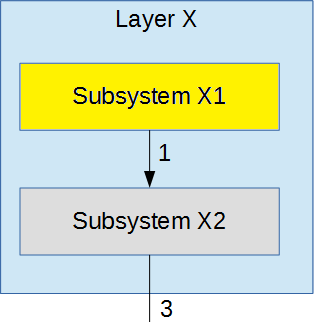
\includegraphics[width=0.60\textwidth]{images/subsystem}
 \caption{Example subsystem description diagram}
\end{figure}

\subsubsection{Assumptions}
These are the following assumptions made about this subsection:
\begin{itemize}
    \item 
\end{itemize}

\subsubsection{Responsibilities}
Each of the responsibilities/features/functions/services of the subsystem as identified in the architectural summary must be expanded to more detailed responsibilities. These responsibilities form the basis for the identification of the finer-grained responsibilities of the layer's internal subsystems. Clearly describe what each subsystem does.

\subsubsection{Subsystem Interfaces}
Each of the inputs and outputs for the subsystem are defined here. Create a table with an entry for each labelled interface that connects to this subsystem. For each entry, describe any incoming and outgoing data elements will pass through this interface.

\begin {table}[H]
\caption {Subsystem interfaces} 
\begin{center}
    \begin{tabular}{ | p{1cm} | p{6cm} | p{3cm} | p{3cm} |}
    \hline
    ID & Description & Inputs & Outputs \\ \hline
    \#xx & Description of the interface/bus & \pbox{3cm}{input 1 \\ input 2} & \pbox{3cm}{output 1}  \\ \hline
    \#xx & Description of the interface/bus & \pbox{3cm}{N/A} & \pbox{3cm}{output 1}  \\ \hline
    \end{tabular}
\end{center}
\end{table}
